\section*{Analiza porównacza wyjaśnień}
W tej sekcji przeprowadzono analizę porównawcą wyjaśnień generowanych przez różne metody XAI: LIME, SHAP i GradCAM.
Oceny zostały dokonane na podstawie IoU oraz na podstawie zmiany pewności modelu.

Analiza została przeprowadzona na trzech poziomach:
\begin{enumerate}
	\item \textbf{Na całym zbiorze danych}, w celu zrozumienia ogólnej skuteczności każdej z metod XAI.
	\item \textbf{Z podziałem na kategorie obrazów}, w celu zbadania, jak różne typy obiektów wpływają na spójność wyjaśnień.
	\item \textbf{W zależności od wielkości obiektów na obrazie}, aby zbadać, czy rozmiar obiektu ma wpływ na spójność wyjaśnień oraz jakie obszary obrazu są istotne dla różnych metod XAI.
\end{enumerate}

Celem tej analizy było zrozumienie, które metody XAI są najbardziej skuteczne w identyfikacji istotnych cech orazów oraz jakie czynniki mogą wpłynąć na spójność i stabilność wyjaśnień generowanych przez metody.
Dzięki temu możliwe jest lepsze zrozumienie mechanizmów działania każdej z metod i ich potencjalnych zastosowań w praktyce.

\subsection*{Analiza na całym zbiorze danych}.

W tej części przeprowadzono analizę porównawczą metod XAI na całym zbiorze danych.
Skupiono się na ocenie Intersection over Union oraz zmianach w pewności modelu po zastosowaniu wyjaśnień.
Celem było zrozumienie, jak skutecznie każda metoda identyfikuje istotne cechy obrazu w kontekście całego zbioru.

\begin{figure}[h]
	\centering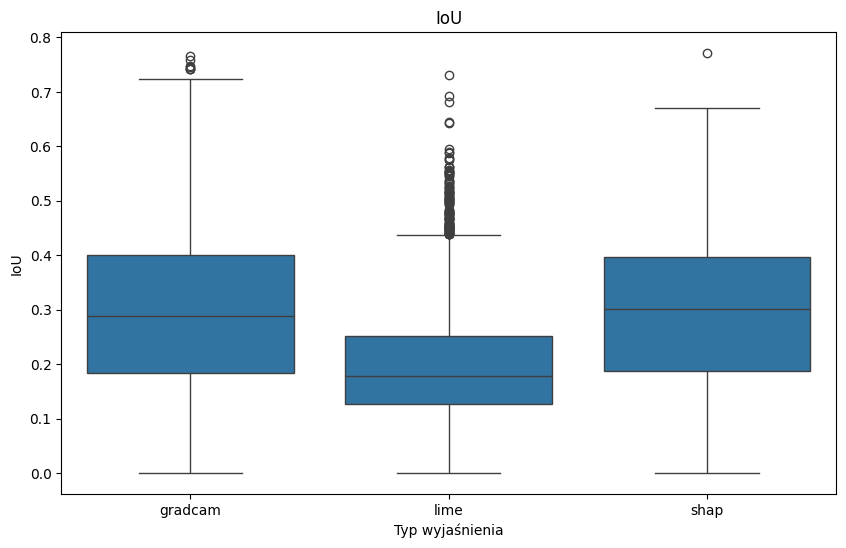
\includegraphics[width=.9\textwidth]{img/base_iou}
	\caption{Wartości IoU  dla stosowanych obrazów}  \label{rys:basiciou}
\end{figure}

\begin{table}[h]
	\centering
	\begin{tabular}{|c|c|c|c|}
		\hline
		\textbf{Metoda XAI}  & \textbf{GradCAM} & \textbf{LIME} & \textbf{SHAP} \\
		\hline
		\textbf{Średnie IoU} & 0.439863         & 0.199370      & 0.292436      \\
		\hline
	\end{tabular}
	\caption{Średnie wartości IoU}
	\label{tab:basiciou}
\end{table}

Wyniki analizy pokazano na wykresie pudełkowym (Rys. \ref{rys:basiciou}), który przedstawia rozkład wartości IoU dla poszczególnych metod XAI.
Dodatkowo, Tabela \ref{tab:basiciou} zawiera średnie wartości IoU dla każdej z metod.

Z wyników wynika, że metoda GradCAM osiągnęła najwyższe średnie wartości IoU, co sugeruje, że generowane przez nią wyjaśnienia najbardziej pokrywają się z rzeczywistymi istotnymi obszarami na obrazach.
Natomiast LIME osiągnęła najniższe średnie IoU.

Te wyniki wskazują, że GradCAM jest najbardziej skuteczny w identyfikacji istotnych cech obrazów na całym zbiorze danych.
Wyższa wartość IoU dla GradCAM może wynikać z doboru niskiego parametru threshold, co powoduje zaznaczenie większego obszaru obrazu.

Metoda LIME, która analizuje lokalne zmiany w predykcji modelu na skutek modyfikacji fragmentów obrazu, wykazała najniższą spójność z rzeczywistymi istotnymi obszarami.
Może to być spowodowane tym, że LIME generuje bardziej szczegółowe, co prowadzi do mniejszej wartości IoU.

Metoda SHAP, która ocenia wpływ każdego piksela na predykcję modelu, uzyskała średnie wartości IoU między GradCAM a LIME, co sugeruje, że generuje wyjaśnienia o umiarkowanej ogólności i precyzji.

\begin{figure}[h]
	\centering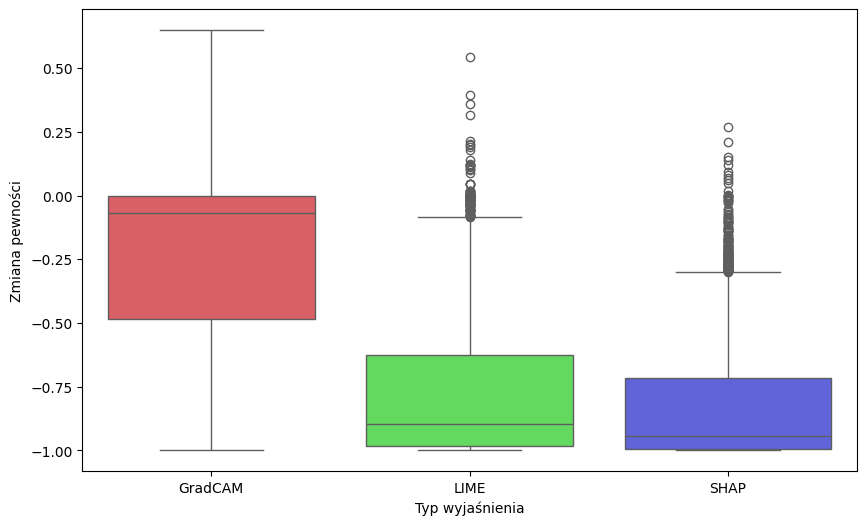
\includegraphics[width=.9\textwidth]{img/base_confidence_exp}
	\caption{Zmiana pewności po pozostawieniu jedynie obszaru wyjaśnienia}  \label{rys:base_confidence_exp}
\end{figure}

\begin{table}[h]
	\centering
	\begin{tabular}{|c|c|c|c|}
		\hline
		\textbf{Metoda XAI}  & \textbf{GradCAM} & \textbf{LIME} & \textbf{SHAP} \\
		\hline
		\textbf{Średnie IoU} & -0.247974        & -0.732920     & -0.58366      \\
		\hline
	\end{tabular}
	\caption{Średni spadek pewności modelu po pozostawieniu jedynie obszaru wyjaśnienia}
	\label{tab:base_confidence_exp}
\end{table}

\begin{table}[h]
	\centering
	\begin{tabular}{|c|c|c|c|}
		\hline
		\textbf{Metoda XAI}  & \textbf{GradCAM} & \textbf{LIME} & \textbf{SHAP} \\
		\hline
		\textbf{Średnie IoU} & 24.8148\%        & 2.2222\%      & 5.6296\%      \\
		\hline
	\end{tabular}
	\caption{Procent przydaków, w których pewność się zwiększyła}
	\label{tab:base_confidence_exp_percent}
\end{table}

Wyniki analizy przedstawiono na wykresie (Rys. \ref{rys:base_confidence_exp}), który ilustruje zmianę pewności modelu po pozostawieniu jedynie obszarów wyjaśnień.
Natomiast Tabela \ref{tab:base_confidence_exp} przedstawia średni spadek pewności modelu dla każdej z metod, natomiast Tabela \ref{tab:base_confidence_exp_percent} pokazuje procent przypadków, w których pewność modelu wzrosła po zastosowaniu wyjaśnień.

Metoda GradCAM wykazała najmniejszy spadek pewności modelu, co sugeruje, że wyjaśnienia generowane przez GradCAM są najbardziej zgodne z rzeczywistymi istotnymi obszarami obrazu.
Średni spadek pewności wyniósł -0.247974, a w 24.8148\% przypadków pewność modelu wzrosła, co jest najwyższym wynikiem spośród analizowanych metod.

Metoda LIME, mimo że generuje szczegółowe wyjaśnienia, wykazała największy spadek pewności modelu (-0.732920) i najniższy procent przypadków ze wzrostem pewności (2.2222\%).
Może to sugerować, że LIME identyfikuje obszary, które nie zawsze są kluczowe dla predykcji modelu.

Metoda SHAP, która ocenia wpływ każdego super pikselu na predykcję, uzyskała średni spadek pewności na poziomie -0.583660 oraz 5.6296\% przypadków ze wzrostem pewności.
Wyniki te wskazują, że SHAP generuje wyjaśnienia o umiarkowanej skuteczności w kontekście identyfikacji istotnych obszarów obrazu.

\begin{figure}[h]
	\centering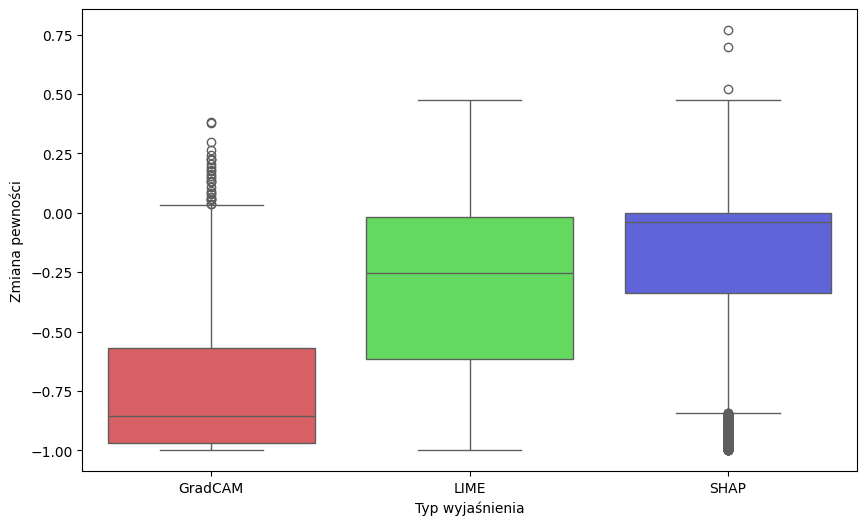
\includegraphics[width=.9\textwidth]{img/base_confidence_no_exp}
	\caption{Zmiana pewności po usunięciu obszaru wyjaśnienia}  \label{rys:base_confidence_no_exp}
\end{figure}

\begin{table}[h]
	\centering
	\begin{tabular}{|c|c|c|c|}
		\hline
		\textbf{Metoda XAI}  & \textbf{GradCAM} & \textbf{LIME} & \textbf{SHAP} \\
		\hline
		\textbf{Średnie IoU} & -0.747604        & -0.404889     & -0.626561     \\
		\hline
	\end{tabular}
	\caption{Średni spadek pewności modelu po usunięciu obszaru wyjaśnienia}
	\label{tab:base_confidence_no_exp}
\end{table}

Wyniki analizy przedstawiono na wykresie (Rys. \ref{rys:base_confidence_no_exp}), który ilustruje zmianę pewności modelu po usunięciu obszaru wyjaśnienia.
Natomiast Tabela \ref{tab:base_confidence_no_exp} przedstawia średni spadek pewności modelu dla każdej z metod.

Metoda GradCAM wykazała największy spadek pewności modelu (-0.747604), co sugeruje, że wyjaśnienia generowane przez GradCAM są najbardziej zgodne z rzeczywistymi istotnymi obszarami obrazu.

Metoda LIME wykazała najmniejszy spadek pewności modelu (-0.404889).
Może to sugerować, że LIME identyfikuje nie wszystkie obszary kluczowe lub identyfikuje nieklucze dla prdykcji modelu obszary.

Metoda SHAP uzyskała średni spadek pewności na poziomie -0.626561.
Wyniki te wskazują, że SHAP generuje wyjaśnienia, które są umiarkowanie skuteczne w kontekście identyfikacji istotnych obszarów obrazu, ale nie są tak trafne jak wyjaśnienia generowane przez GradCAM.

\subsection*{Analiza z podziałem na kategorie obrazu}

W tej części dokonano analizy porównawczej metod XAI z uwzględnieniem różnych kategorii obrazów.
Porównano skuteczność wyjaśnień generowanych przez LIME, SHAP i GradCAM dla różnych klas.
Celem była ocena, jak metody radzą sobie w kontekście specyficznych rodzajów obrazów.

\begin{figure}[h]
	\centering
	\begin{subfigure}[b]{0.3\textwidth}
		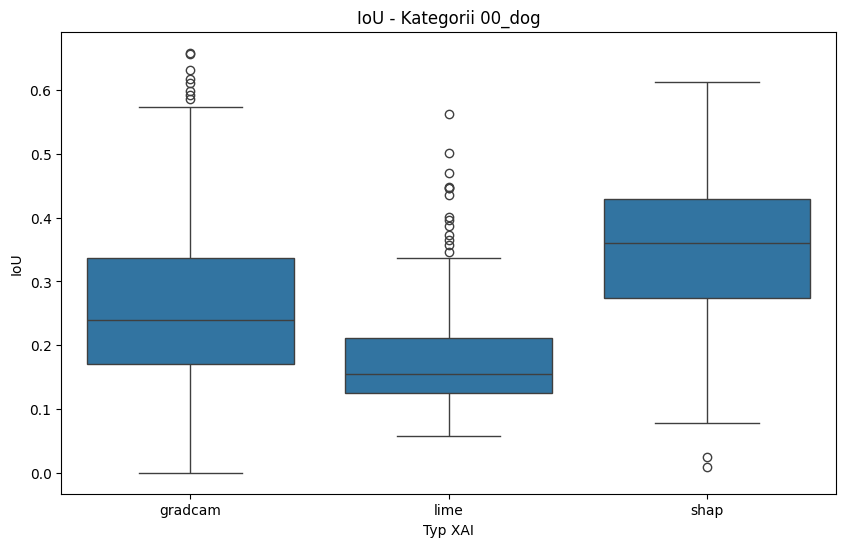
\includegraphics[width=.9\textwidth]{img/base_iou_dog}
		\caption{Dog}
	\end{subfigure}
	\begin{subfigure}[b]{0.3\textwidth}
		\centering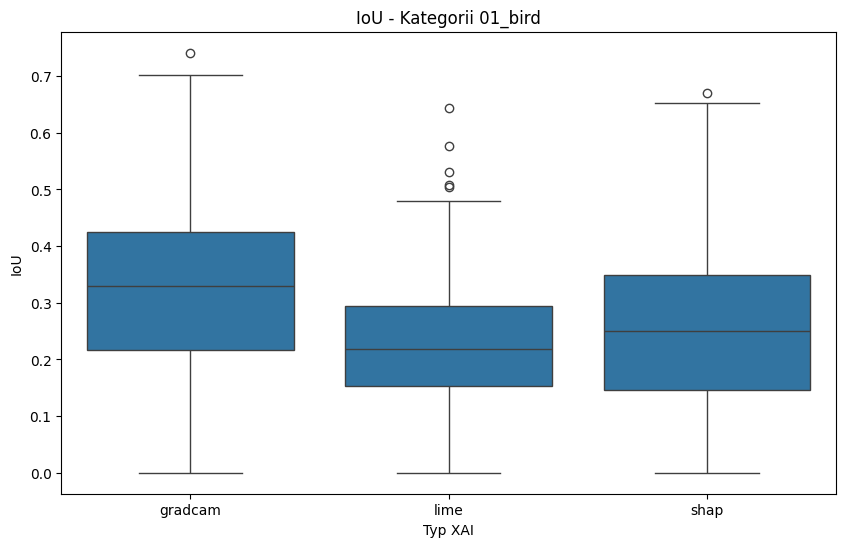
\includegraphics[width=.9\textwidth]{img/base_iou_bird}
		\caption{Bird}
	\end{subfigure}
	\begin{subfigure}[b]{0.3\textwidth}
		\centering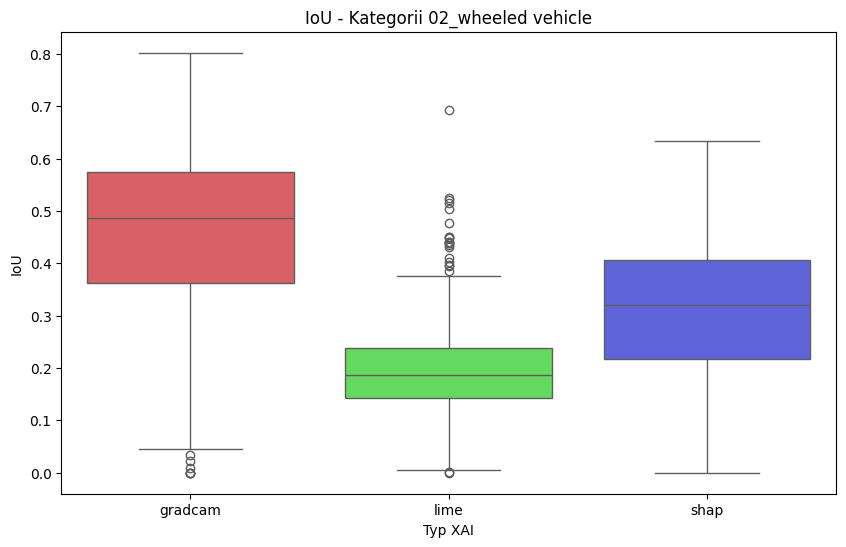
\includegraphics[width=.9\textwidth]{img/base_iou_vehicle}
		\caption{Vehicle}
	\end{subfigure}
	\begin{subfigure}[b]{0.3\textwidth}
		\centering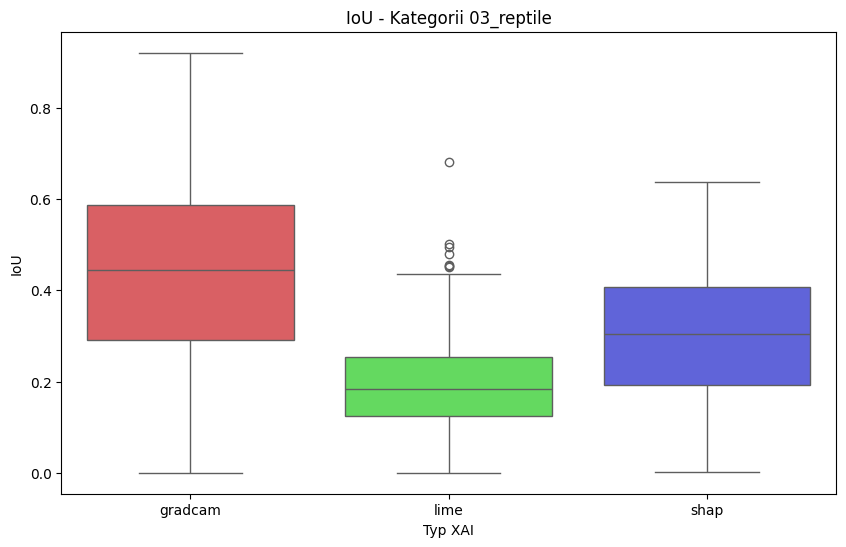
\includegraphics[width=.9\textwidth]{img/base_iou_reptile}
		\caption{Reptile}
	\end{subfigure}
	\begin{subfigure}[b]{0.3\textwidth}
		\centering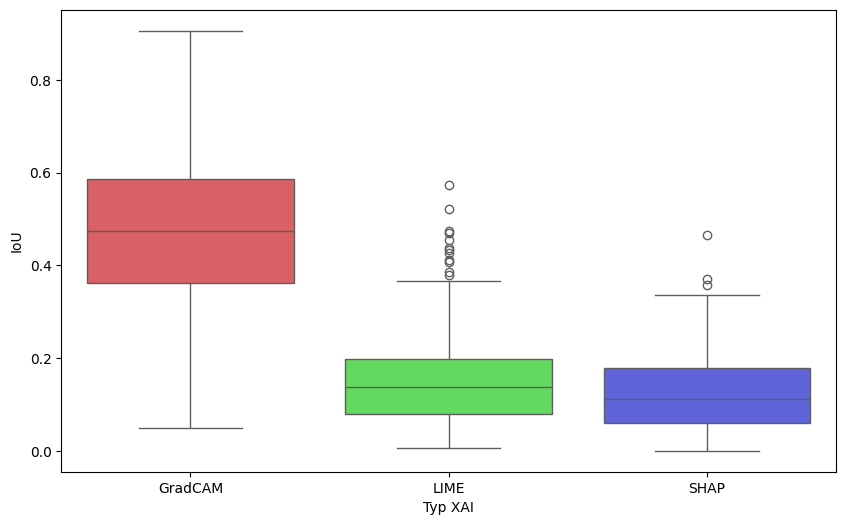
\includegraphics[width=.9\textwidth]{img/base_iou_carnivore}
		\caption{Carnivore}
	\end{subfigure}
	\begin{subfigure}[b]{0.3\textwidth}
		\centering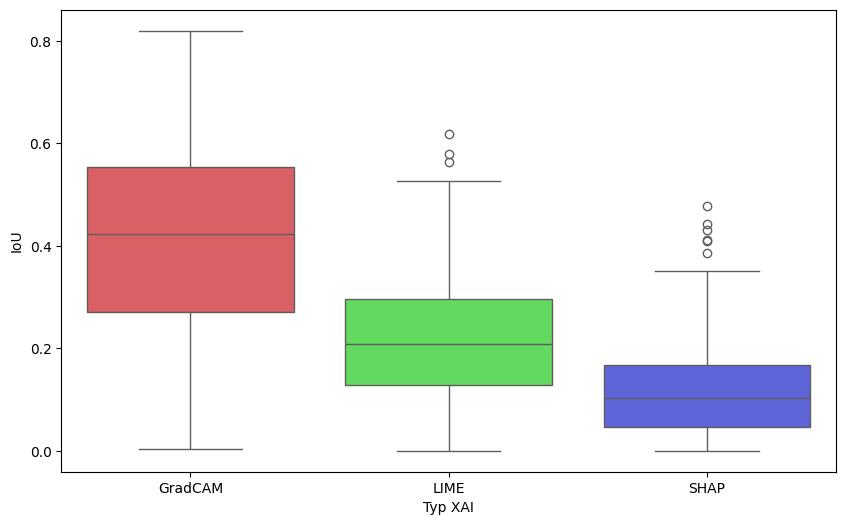
\includegraphics[width=.9\textwidth]{img/base_iou_insect}
		\caption{Insect}
	\end{subfigure}
	\begin{subfigure}[b]{0.3\textwidth}
		\centering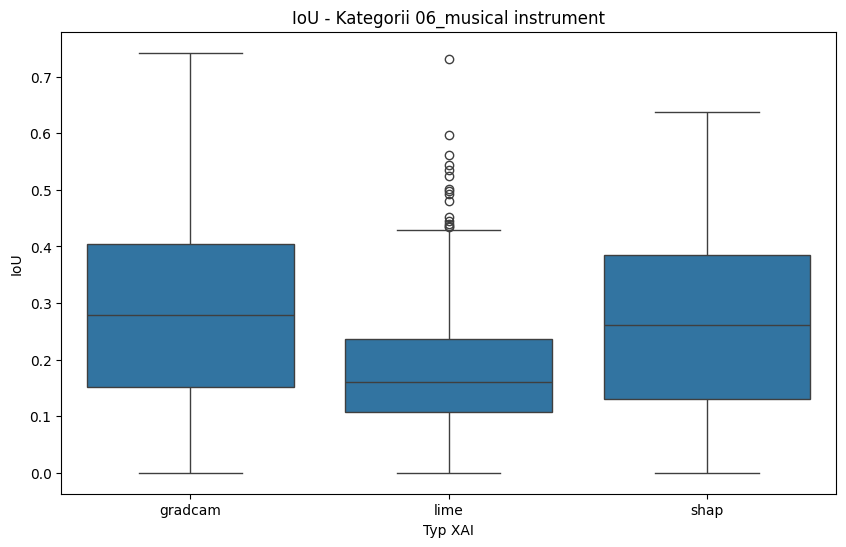
\includegraphics[width=.9\textwidth]{img/base_iou_music}
		\caption{Instrument}
	\end{subfigure}
	\begin{subfigure}[b]{0.3\textwidth}
		\centering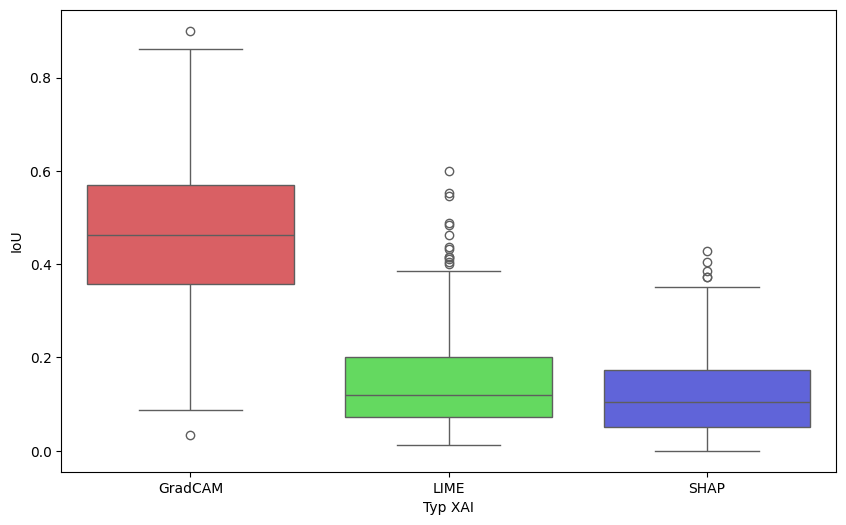
\includegraphics[width=.9\textwidth]{img/base_iou_primate}
		\caption{Primate}
	\end{subfigure}
	\begin{subfigure}[b]{0.3\textwidth}
		\centering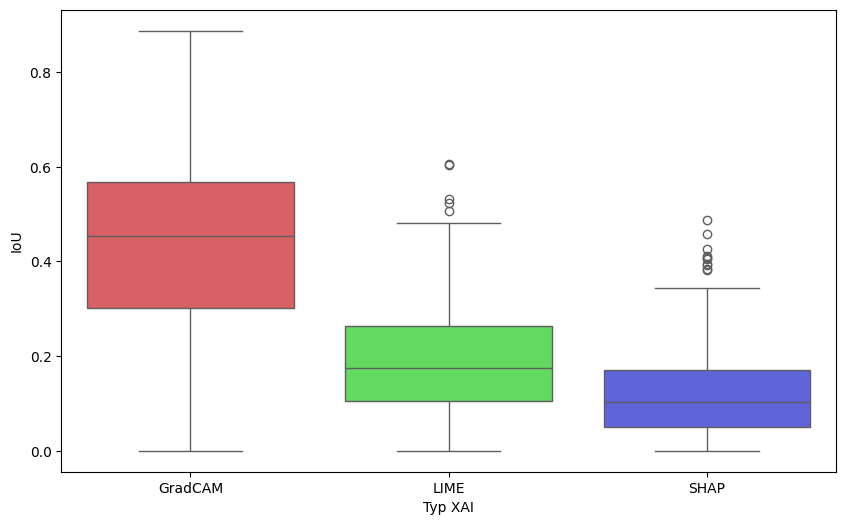
\includegraphics[width=.9\textwidth]{img/base_iou_fish}
		\caption{Fish}
	\end{subfigure}
	\caption{Wartości IoU dla różnych kategorii}
	\label{rys:base_iou_category}
\end{figure}

\begin{table}[h]
	\centering
	\begin{tabular}{|c|c|c|c|}
		\hline
		\textbf{Kategoria}           & \textbf{GradCAM} & \textbf{LIME} & \textbf{SHAP} \\
		\hline
		\textbf{Pies}                & 0.467134         & 0.174455      & 0.351659      \\
		\hline
		\textbf{Ptak}                & 0.428416         & 0.232156      & 0.253825      \\
		\hline
		\textbf{Pojazd na kołach}    & 0.459880         & 0.199560      & 0.308771      \\
		\hline
		\textbf{Gad}                 & 0.436193         & 0.198447      & 0.302146      \\
		\hline
		\textbf{Mięsożerca}          & 0.468916         & 0.173762      & 0.335634      \\
		\hline
		\textbf{Insekt}              & 0.410650         & 0.252195      & 0.255142      \\
		\hline
		\textbf{Instrument muzyczny} & 0.394289         & 0.182606      & 0.261536      \\
		\hline
		\textbf{Naczelny}            & 0.465292         & 0.165912      & 0.332052      \\
		\hline
		\textbf{Ryba}                & 0.427992         & 0.215236      & 0.261161      \\
		\hline
	\end{tabular}
	\caption{IoU dla kategorii}
	\label{tab:base_iou_category}
\end{table}

Wyniki analizy IoU w zależności od kategorii obrazów przedstawiono na wykresach (Rys. \ref{rys:base_iou_category}) oraz w Tabeli \ref{tab:base_iou_category}, która zawiera średnie wartości IoU dla poszczególnych metod XAI i kategorii.

Z analizy wynika, że metoda GradCAM osiągnęła najwyższe średnie wartości IoU we wszystkich kategoriach, co wskazuje na jej najwyższą skuteczność w identyfikacji istotnych cech obrazów niezależnie od ich rodzaju.
Najlepsze wyniki gradcam osiągnął dla kategorii Pies, Pojazd na kołach, Mięsożerca oraz Naczelny.
Natomias najgorsze wyniki osiągneł dla kategorii Insstrument muzyczny oraz Insekt.

Metoda SHAP, mimo że generalnie osiągnęła średnie wartości IoU pomiędzy GradCAM a LIME, wykazała szczególną skuteczność w kategoriach Pies, Mięsożerca i Naczelny.
Natomiast najgorzej porodził sobie z kategoriamii Ptak i Insekt.

Metoda LIME miała najniższe wartości IoU we wszystkich kategoriach.
Wyniki kategorii Insekt dla LIME, były podobne do wyników SHAPA, co sugeruje, że w tej konkretnej kategorii obie metody osiągneły porównywalne wyniki.
Najgorsze wyniki uzyskał dla kategorii Naczelny.

Ogólnie rzecz biorąc, wyniki te sugerują, że skuteczność metod XAI różni się w zależności od rodzaju obrazów, a wybór odpowiedniej metody powinien uwzględniać specyfikę analizowanej kategorii.

\begin{figure}[h]
	\centering
	\begin{subfigure}[b]{0.3\textwidth}
		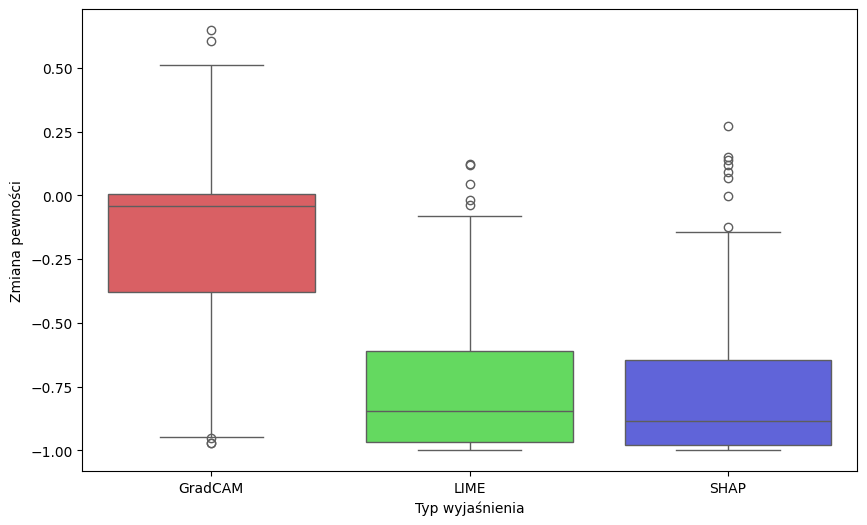
\includegraphics[width=.9\textwidth]{img/base_confidence_exp_dog}
		\caption{Dog}  \label{rys:base_confidence_exp_dog}
	\end{subfigure}
	\begin{subfigure}[b]{0.3\textwidth}
		\centering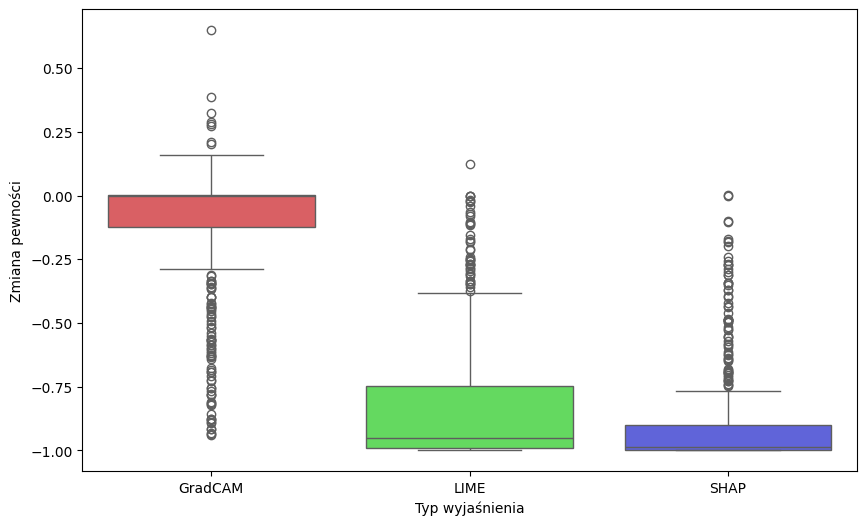
\includegraphics[width=.9\textwidth]{img/base_confidence_exp_bird}
		\caption{Bird}  \label{rys:base_confidence_exp_bird}
	\end{subfigure}
	\begin{subfigure}[b]{0.3\textwidth}
		\centering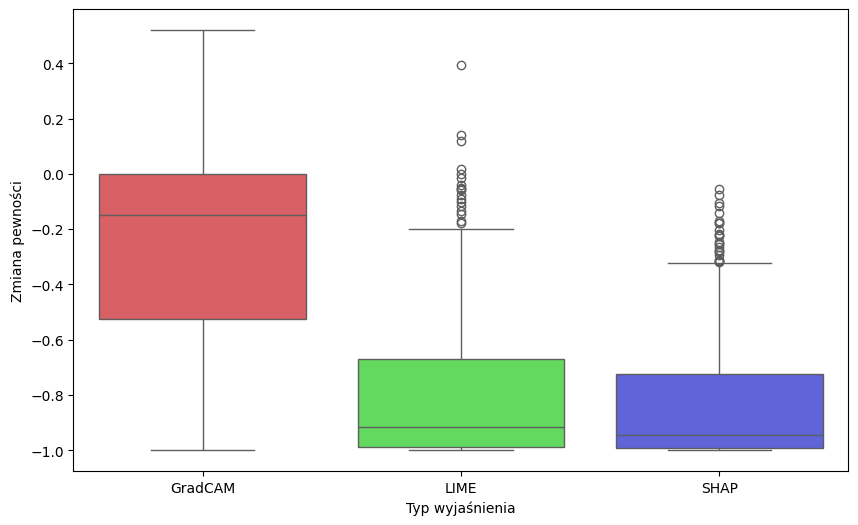
\includegraphics[width=.9\textwidth]{img/base_confidence_exp_vehicle}
		\caption{Vehicle}  \label{rys:base_confidence_exp_vehicle}
	\end{subfigure}
	\begin{subfigure}[b]{0.3\textwidth}
		\centering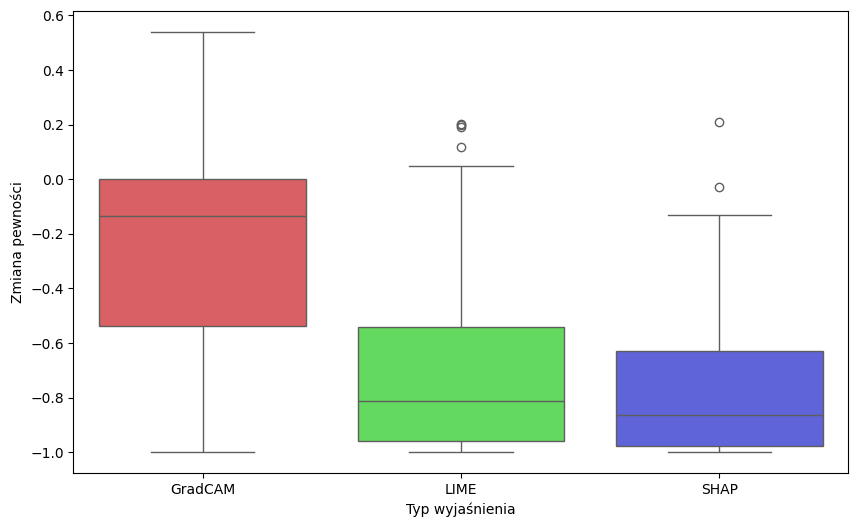
\includegraphics[width=.9\textwidth]{img/base_confidence_exp_reptile}
		\caption{Reptile}  \label{rys:base_confidence_exp_reptile}
	\end{subfigure}
	\begin{subfigure}[b]{0.3\textwidth}
		\centering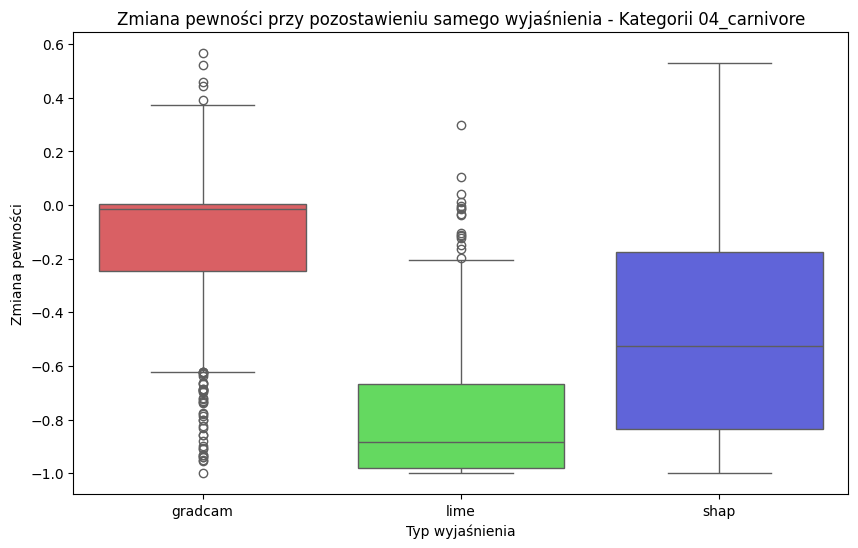
\includegraphics[width=.9\textwidth]{img/base_confidence_exp_carnivore}
		\caption{Carnivore}  \label{rys:base_confidence_exp_carnivore}
	\end{subfigure}
	\begin{subfigure}[b]{0.3\textwidth}
		\centering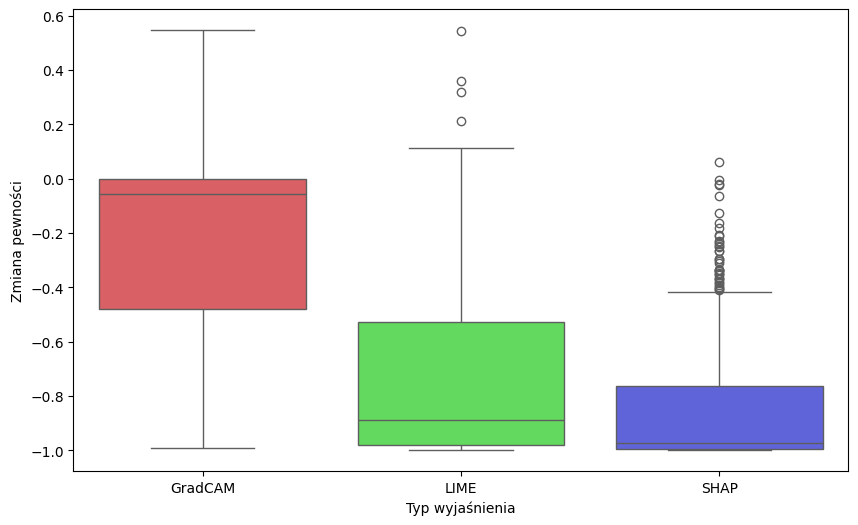
\includegraphics[width=.9\textwidth]{img/base_confidence_exp_insect}
		\caption{Insect}  \label{rys:base_confidence_exp_insect}
	\end{subfigure}
	\begin{subfigure}[b]{0.3\textwidth}
		\centering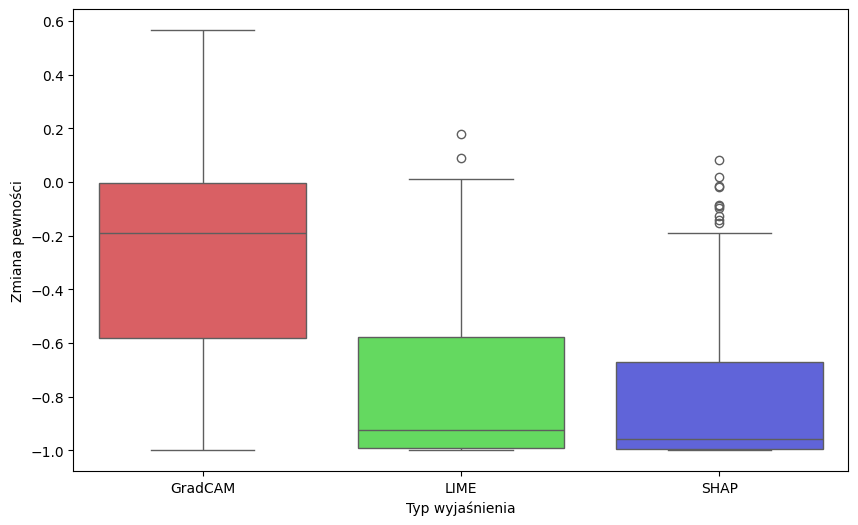
\includegraphics[width=.9\textwidth]{img/base_confidence_exp_music}
		\caption{Instrument}  \label{rys:base_confidence_exp_music}
	\end{subfigure}
	\begin{subfigure}[b]{0.3\textwidth}
		\centering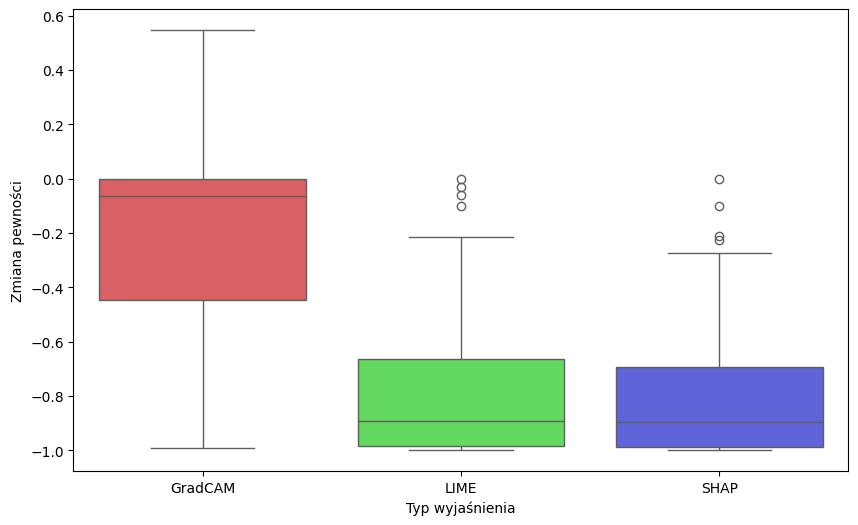
\includegraphics[width=.9\textwidth]{img/base_confidence_exp_primate}
		\caption{Primate}  \label{rys:base_confidence_exp_primate}
	\end{subfigure}
	\begin{subfigure}[b]{0.3\textwidth}
		\centering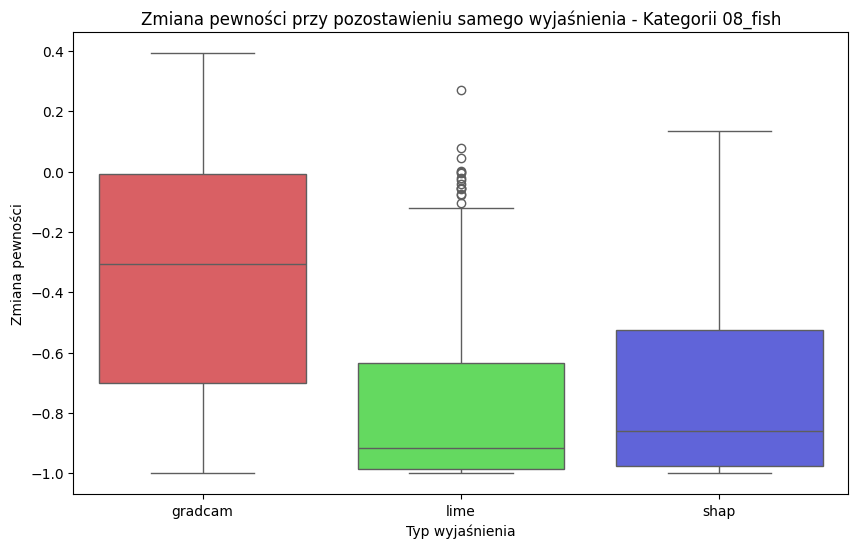
\includegraphics[width=.9\textwidth]{img/base_confidence_exp_fish}
		\caption{Fish}  \label{rys:base_confidence_exp_fish}
	\end{subfigure}
	\caption{Zmiana pewności po pozostawieniu jedynie obszatu wyjaśnienia dla różnych kategorii}
	\label{rys:base_confidence_exp_category}
\end{figure}

\begin{table}[h]
	\centering
	\begin{tabular}{|c|c|c|c|}
		\hline
		\textbf{Kategoria}           & \textbf{GradCAM} & \textbf{LIME} & \textbf{SHAP} \\
		\hline
		\textbf{Pies}                & -0.203837        & -0.730913     & -0.523232     \\
		\hline
		\textbf{Ptak}                & -0.126917        & -0.695752     & -0.528825     \\
		\hline
		\textbf{Pojazd na kołami}    & -0.283471        & -0.766767     & -0.626653     \\
		\hline
		\textbf{Gad}                 & -0.281027        & -0.703908     & -0.597428     \\
		\hline
		\textbf{Mięsożerca}          & -0.165199        & -0.781692     & -0.510289     \\
		\hline
		\textbf{Insekt}              & -0.244699        & -0.630861     & -0.594027     \\
		\hline
		\textbf{Instrument muzyczny} & -0.315661        & -0.733294     & -0.602684     \\
		\hline
		\textbf{Naczelny}            & -0.236171        & -0.765780     & -0.557879     \\
		\hline
		\textbf{Ryba}                & -0.374784        & -0.787316     & -0.711981     \\
		\hline
	\end{tabular}
	\caption{Średni spadek pewności modelu po pozostawieniu jedynie obszaru wyjaśnienia dla kategorii}
	\label{tab:category_confidence_exp}
\end{table}

\begin{table}[h]
	\centering
	\begin{tabular}{|c|c|c|c|}
		\hline
		\textbf{Kategoria}           & \textbf{GradCAM} & \textbf{LIME} & \textbf{SHAP} \\
		\hline
		\textbf{Pies}                & 32.8889\%        & 2.2222\%      & 7.1111\%      \\
		\hline
		\textbf{Ptak}                & 35.3333\%        & 4.6667\%      & 6.4444\%      \\
		\hline
		\textbf{Pojazd na kołami}    & 20.0000\%        & 0.4444\%      & 4.4444\%      \\
		\hline
		\textbf{Gad}                 & 25.5556\%        & 1.5556\%      & 6.8889\%      \\
		\hline
		\textbf{Mięsożerca}          & 31.5556\%        & 0.8889\%      & 6.8889\%      \\
		\hline
		\textbf{Insekt}              & 23.1111\%        & 6.2222\%      & 5.1111\%      \\
		\hline
		\textbf{Instrument muzyczny} & 14.8889\%        & 1.7778\%      & 4.4444\%      \\
		\hline
		\textbf{Naczelny}            & 27.3333\%        & 1.3333\%      & 6.2222\%      \\
		\hline
		\textbf{Ryba}                & 12.6667\%        & 0.8889\%      & 3.1111\%      \\
		\hline
	\end{tabular}
	\caption{Procent przypadków, w których pewność się zwiększyła dla kategorii}
	\label{tab:category_confidence_exp_percent}
\end{table}

Wyniki analizy zmiany pewności po pozostawieniu jedynie obszaru wyjaśnienia dla różnych kategorii obrazów przedstawiono na wykresach (Rys. \ref{rys:base_confidence_exp_category}) oraz w Tabelach \ref{tab:category_confidence_exp} i \ref{tab:category_confidence_exp_percent}, które zawierają średni spadek pewności modelu oraz procent przypadków, w których pewność modelu się zwiększyła po usunięciu obszarów uznanych przez metodę za nieistotne.

Z analizy wynika, że metoda GradCAM konsekwentnie powoduje najmniejszy spadek pewności modelu w różnych kategoriach obrazów, co wskazuje na jej skuteczność w zachowywaniu kluczowych informacji przy pozostawieniu jedynie obszaru wyjaśnienia.
Najmniejszy spadek pewności odnotowano w kategorii Ptak, a największy w kategorii Ryba.

Metoda SHAP wykazała mniejsze spadki pewności w kategoriach Pies, Ptak i Mięsożerca, większe spadki dla kategorii Ryba.

Metoda LIME miała najniższe wartości we wszystkich kategoriach, co wskazuje na największy spadek pewności modelu. Największy spadek pewności zaobserwowano w kategorii Ryba i Mięsożerca, a najmniejszy w kategorii Ptak.

Dodatkowo, analiza procentu przypadków, w których pewność modelu się zwiększyła, pokazuje, że GradCAM również w tej mierze osiąga lepsze wyniki.
W kategorii Ptak aż 35.3333\% przypadków odnotowało wzrost pewności modelu, co jest najwyższą wartością spośród wszystkich metod i kategorii.
LIME pomimo gorszego wyniku zarówno IoU jak i średniego spadku pewności posiadał większy procent przypadków zwiększenia się pewności dla kategorii Insekt od SHAP.

\begin{figure}[h]
	\centering
	\begin{subfigure}[b]{0.3\textwidth}
		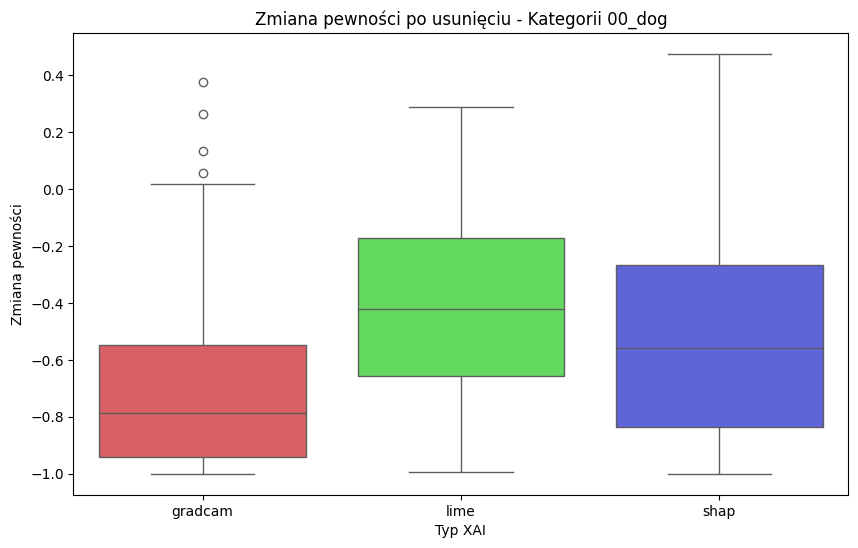
\includegraphics[width=.9\textwidth]{img/base_confidence_no_exp_dog}
		\caption{Dog}  \label{rys:base_confidence_no_exp_dog}
	\end{subfigure}
	\begin{subfigure}[b]{0.3\textwidth}
		\centering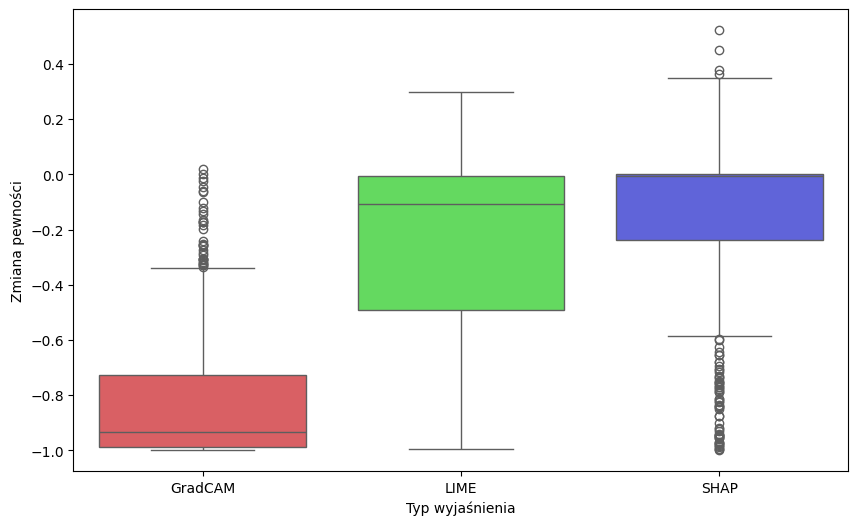
\includegraphics[width=.9\textwidth]{img/base_confidence_no_exp_bird}
		\caption{Bird}  \label{rys:base_confidence_no_exp_bird}
	\end{subfigure}
	\begin{subfigure}[b]{0.3\textwidth}
		\centering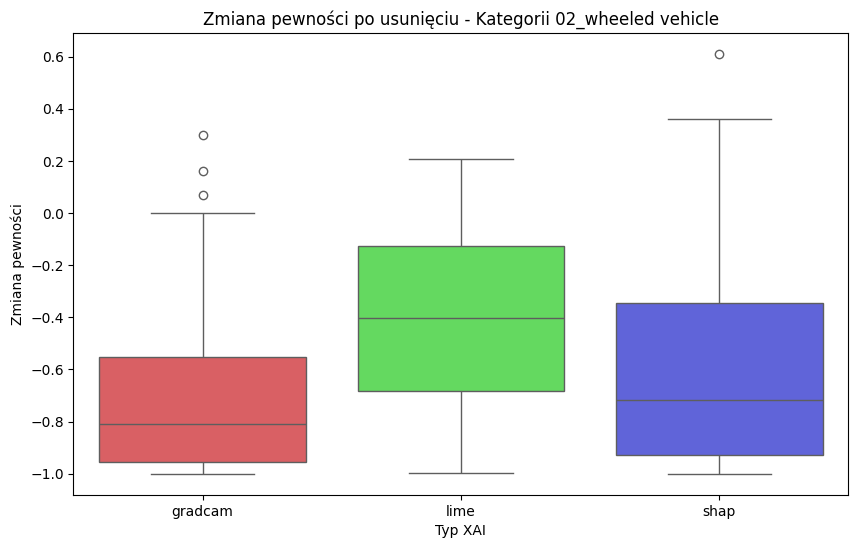
\includegraphics[width=.9\textwidth]{img/base_confidence_no_exp_vehicle}
		\caption{Vehicle}  \label{rys:base_confidence_no_exp_vehicle}
	\end{subfigure}
	\begin{subfigure}[b]{0.3\textwidth}
		\centering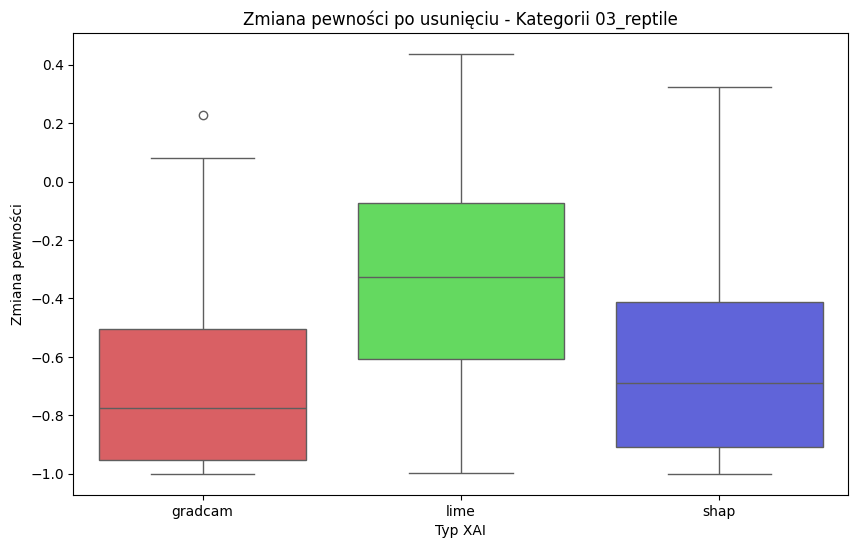
\includegraphics[width=.9\textwidth]{img/base_confidence_no_exp_reptile}
		\caption{Reptile}  \label{rys:base_confidence_no_exp_reptile}
	\end{subfigure}
	\begin{subfigure}[b]{0.3\textwidth}
		\centering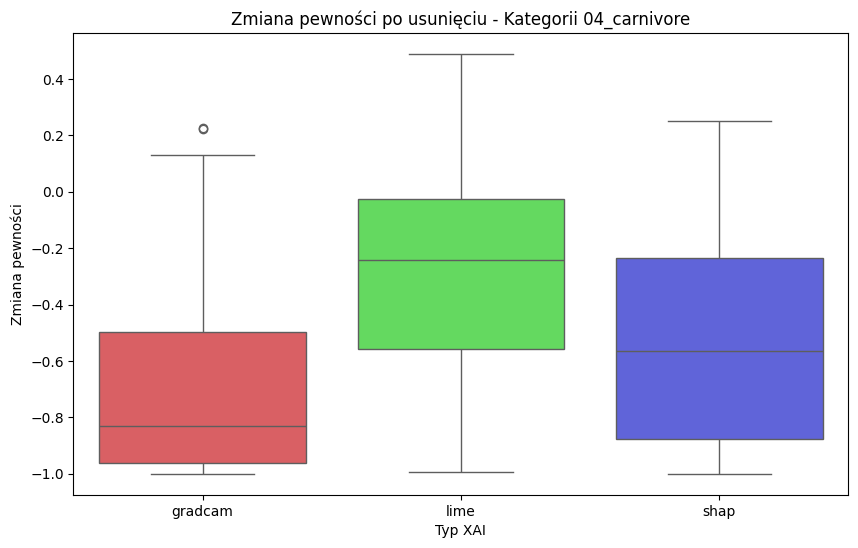
\includegraphics[width=.9\textwidth]{img/base_confidence_no_exp_carnivore}
		\caption{Carnivore}  \label{rys:base_confidence_no_exp_carnivore}
	\end{subfigure}
	\begin{subfigure}[b]{0.3\textwidth}
		\centering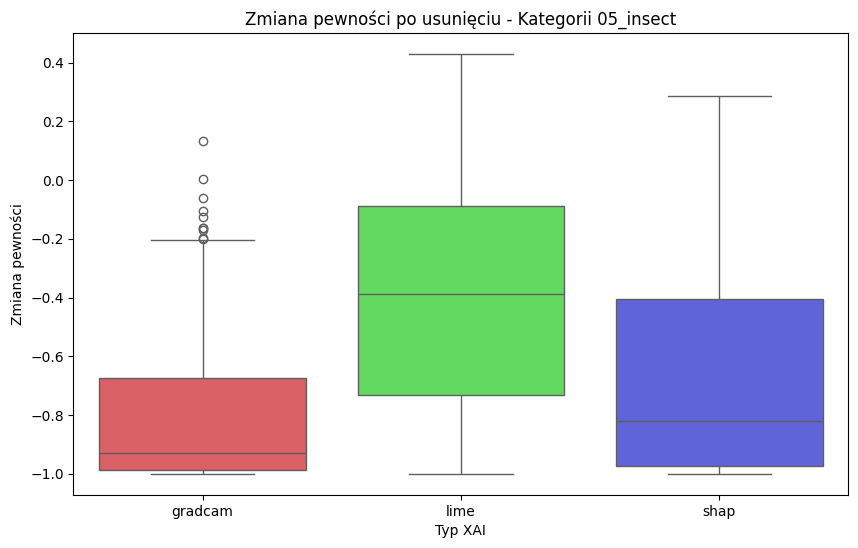
\includegraphics[width=.9\textwidth]{img/base_confidence_no_exp_insect}
		\caption{Insect}  \label{rys:base_confidence_no_exp_insect}
	\end{subfigure}
	\begin{subfigure}[b]{0.3\textwidth}
		\centering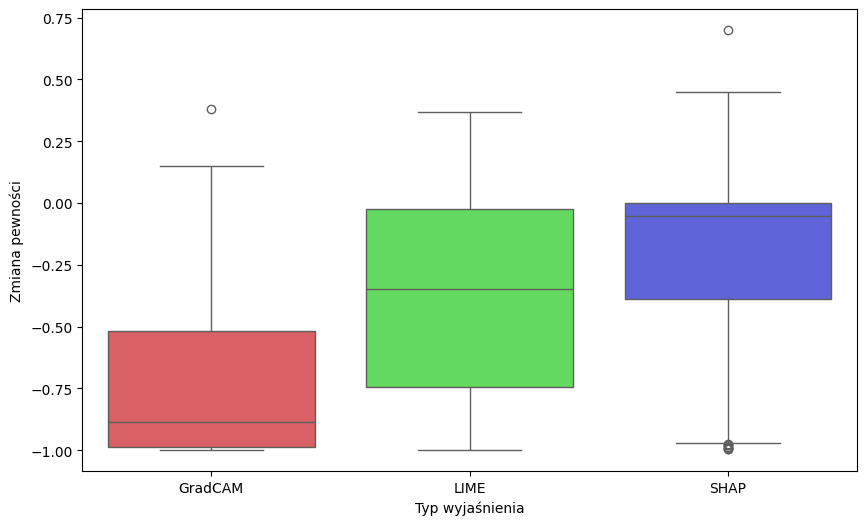
\includegraphics[width=.9\textwidth]{img/base_confidence_no_exp_music}
		\caption{Instrument}  \label{rys:base_confidence_no_exp_music}
	\end{subfigure}
	\begin{subfigure}[b]{0.3\textwidth}
		\centering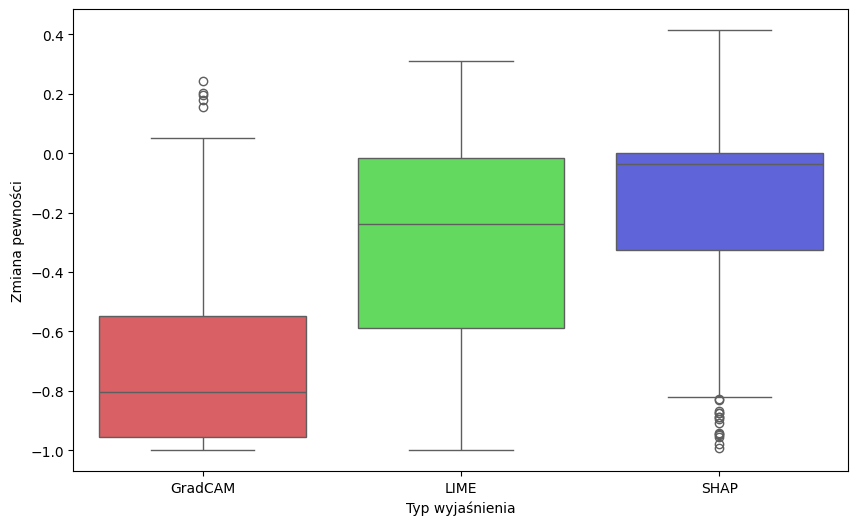
\includegraphics[width=.9\textwidth]{img/base_confidence_no_exp_primate}
		\caption{Primate}  \label{rys:base_confidence_no_exp_primate}
	\end{subfigure}
	\begin{subfigure}[b]{0.3\textwidth}
		\centering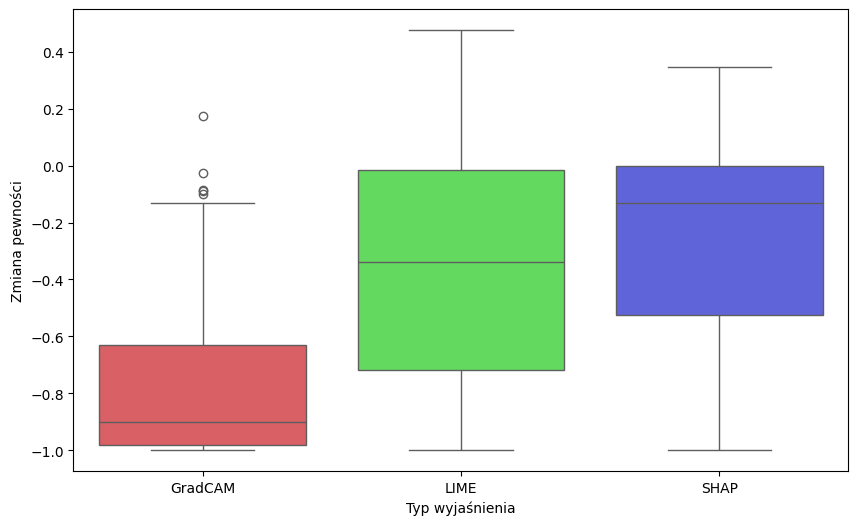
\includegraphics[width=.9\textwidth]{img/base_confidence_no_exp_fish}
		\caption{Fish}  \label{rys:base_confidence_no_exp_fish}
	\end{subfigure}
	\caption{Zmiana pewności po usunięciu obszaru wyjaśnienia dla różnych kategorii}
	\label{rys:category_confidence_no_exp}
\end{figure}

\begin{table}[h]
	\centering
	\begin{tabular}{|c|c|c|c|}
		\hline
		\textbf{Kategoria}           & \textbf{GradCAM} & \textbf{LIME} & \textbf{SHAP} \\
		\hline
		\textbf{Pies}                & -0.712184        & -0.417865     & -0.537021     \\
		\hline
		\textbf{Ptak}                & -0.815407        & -0.434966     & -0.675336     \\
		\hline
		\textbf{Pojazd na kołami}    & -0.731519        & -0.413569     & -0.622449     \\
		\hline
		\textbf{Gad}                 & -0.709709        & -0.368300     & -0.614917     \\
		\hline
		\textbf{Mięsożerca}          & -0.709833        & -0.316740     & -0.542409     \\
		\hline
		\textbf{Insekt}              & -0.802191        & -0.421774     & -0.676712     \\
		\hline
		\textbf{Instrument muzyczny} & -0.729714        & -0.423949     & -0.627190     \\
		\hline
		\textbf{Naczelny}            & -0.730957        & -0.368148     & -0.621441     \\
		\hline
		\textbf{Ryba}                & -0.786923        & -0.478694     & -0.721575     \\
		\hline
	\end{tabular}
	\caption{Średni spadek pewności modelu po usunięciu obszaru wyjaśnienia dla kategorii}
	\label{tab:category_confidence_no_exp}
\end{table}

Wyniki analizy zmiany pewności po usunięciu obszaru wyjaśnień dla różnych kategorii obrazów przedstawiono na wykresach (Rys. \ref{rys:category_confidence_no_exp}) oraz w Tabelach \ref{tab:category_confidence_no_exp}, które zawierają średni spadek pewności modelu.

Z analizy wynika, że metoda LIME powoduje najmniejszy spadek pewności modelu po usunięciu obszaru wyjaśnienia w większości kategorii obrazów, co sugeruje, że generowane przez nią wyjaśnienia są mniej istotne dla decyzji modelu.
Najmniejszy spadek pewności odnotowano w kategorii Mięsożerca, a największy w kategorii Ptak.

Metoda SHAP wykazuje średnie wartości spadku pewności pomiędzy LIME a GradCAM.
Warto zauważyć, że najmniejszy spadek pewności modelu po usunięciu obszaru wyjaśnienia dla SHAP wystąpił w kategorii Mięsożerca.

Metoda GradCAM wykazuje największe spadki pewności modelu po usunięciu obszaru wyjaśnienia we wszystkich kategoriach obrazów.
Największy spadek pewności odnotowano w kategorii Ptak, co wskazuje na to, że obszary wyjaśnień generowanych przez GradCAM są kluczowe dla decyzji modelu w przypadku obrazów tej kategorii.

Podsumowując, LIME powoduje najmniejszy spadek pewności modelu po usunięciu obszaru wyjaśnienia, co sugeruje, że generowane przez nią wyjaśnienia są mniej istotne dla decyzji modelu.
Metoda SHAP osiąga średnie wyniki pomiędzy LIME a GradCAM, a GradCAM wykazuje największe spadki pewności modelu, co sugeruje, że obszary wyjaśnień generowanych przez tę metodę są kluczowe dla decyzji modelu.

\subsection*{Analiza w zależności od wielkość obiektu}

\textbf{Analiza w zależności od wielkości obiektu}.
Przeanalizowano, jak metody XAI radziły sobie w identyfikacji istotnych cech obrazów w zależności od wielkości obiektów.
Porównano wyniki IoU oraz zmiany pewności modelu dla małych, średnich oraz dużych obiektów.
Celem było zrozumienie, jak wielkość obiektu wpływa na skuteczność wyjaśnień generowanych przez różne metody.

\begin{figure}[h]
	\centering
	\begin{subfigure}[b]{0.3\textwidth}
		\centering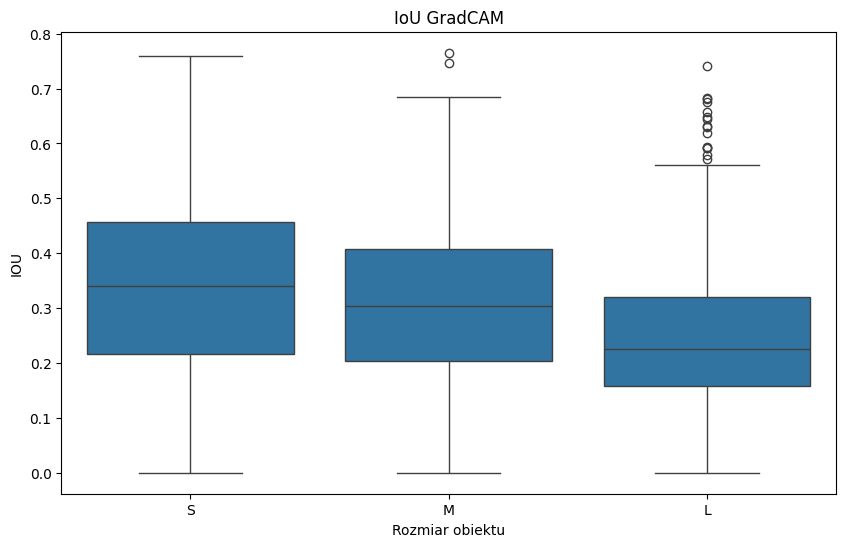
\includegraphics[width=.9\textwidth]{img/size_iou_gradcam}
		\caption{GradCAM}  \label{rys:size_iou_gradcam}
	\end{subfigure}
	\begin{subfigure}[b]{0.3\textwidth}
		\centering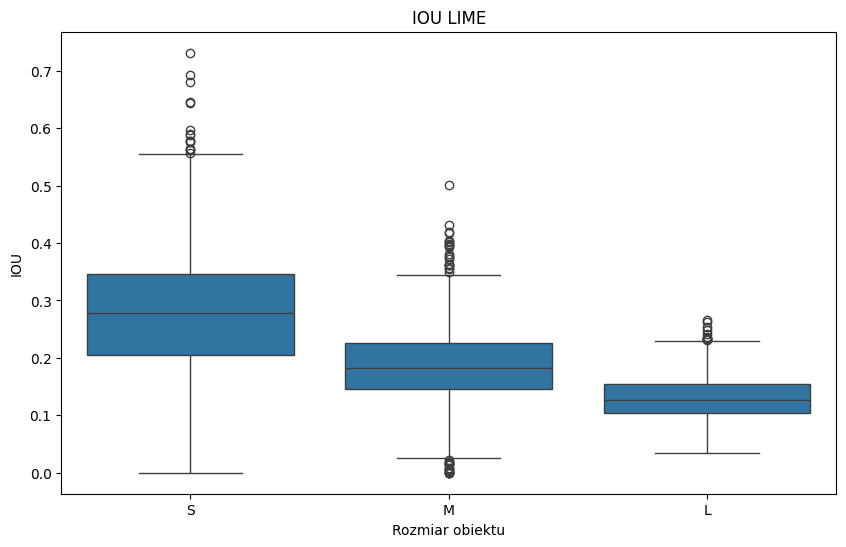
\includegraphics[width=.9\textwidth]{img/size_iou_lime}
		\caption{LIME}  \label{rys:size_iou_lime}
	\end{subfigure}
	\begin{subfigure}[b]{0.3\textwidth}
		\centering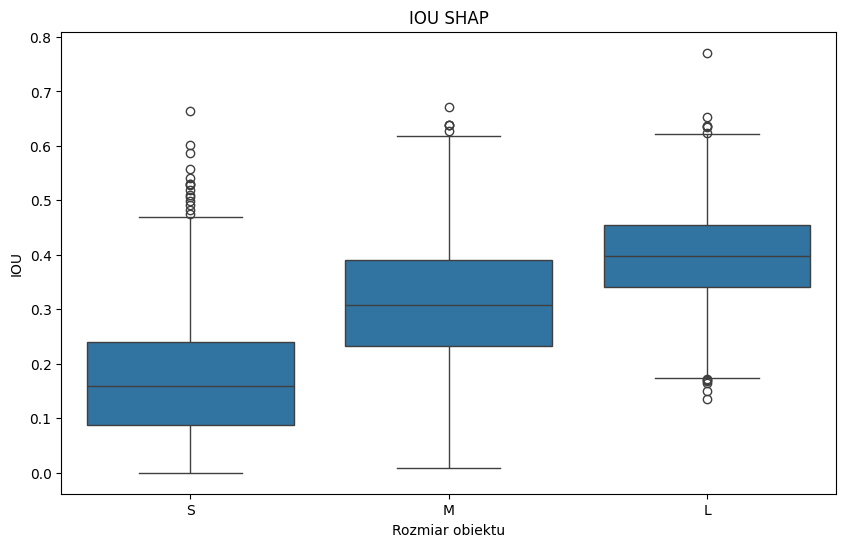
\includegraphics[width=.9\textwidth]{img/size_iou_shap}
		\caption{SHAP}  \label{rys:size_iou_shap}
	\end{subfigure}
	\caption{Wartości IoU w zależności od rozmiaru obiektu na obrazie}
	\label{rys:size_iou}
\end{figure}

\begin{table}[h]
	\centering
	\begin{tabular}{|c|c|c|c|}
		\hline
		\textbf{Rozmiar} & \textbf{GradCAM} & \textbf{LIME} & \textbf{SHAP} \\
		\hline
		\textbf{Mały}    & 0.345227         & 0.276572      & 0.171397      \\
		\hline
		\textbf{Średni}  & 0.477717         & 0.186679      & 0.314621      \\
		\hline
		\textbf{Duży}    & 0.497586         & 0.131633      & 0.396037      \\
		\hline
	\end{tabular}
	\caption{Średnie wartości IoU w zależności od rozmiaru obiektu na obrazie}
	\label{tab:size_iou}
\end{table}

Wyniki analizy IoU dla różnych wielkości obiektów obrazów przedstawiono na wykresach (Rys. \ref{rys:size_iou}) oraz w Tabeli \ref{tab:size_iou}, która zawiera średnie wartości IoU.

GradCAM osiągnął najlepsze wyniki IoU dla dużych obiektów.
Skuteczność GradCAM jest proporcjonalna do wielkości obiektu: im większy obiekt, tym wyższa wartość IoU.
Wskazuje to, że GradCAM lepiej identyfikuje kluczowe obszary na obrazach zawierające większe obiekty.
Może to być spowodowane niską rozdzielczością wyjaśnień wynikającą z wielkości ostatniej warstwy konwolucyjnej w ResNet50.

LIME osiągnął najniższą wartość IoU dla dużych obiektów.
Skuteczność LIME jest odwrotnie proporcjonalna do wielkości obiektu:  im większy obiekt, tym niższa wartość IoU.
Wskazuje to, że LIME lepiej radzi sobie z mniejszymi obiektami, mając trudności z identyfikacją kluczowych cech na większych obiektach.
Może to być spowodowane ustawionymi parametrami, gdyż LIME jest wysoce wrażliwy na parametry.

SHAP osiągał najlepsze wyniki dla dużych obiektów.
Skuteczność SHAP również była proporcjonalna do wielkości obiektu: im większy obiekt tym wyższa wartość IoU.
Podobnie jak GradCAM, SHAP lepiej identyfikuje istotne obszary dla większych obiektów, choć jego skuteczność nie jest tak wysoka jak dla GradCAM.

\textbf{Zmiana pewności przy pozostawieniu samego wyjaśnienia}
\begin{figure}[h]
	\centering
	\begin{subfigure}[b]{0.3\textwidth}
		\centering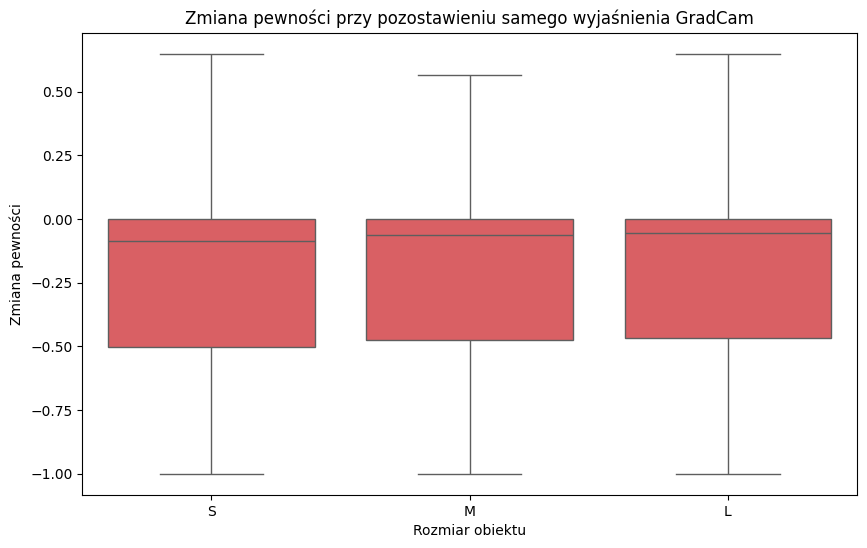
\includegraphics[width=.9\textwidth]{img/size_confidence_exp_gradcam}
		\caption{GradCAM}  \label{rys:size_confidence_mask_gradcam}
	\end{subfigure}
	\begin{subfigure}[b]{0.3\textwidth}
		\centering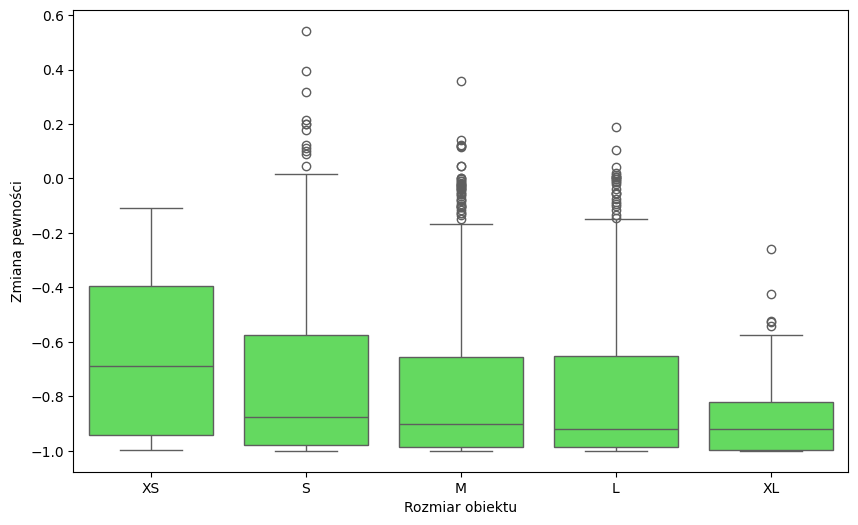
\includegraphics[width=.9\textwidth]{img/size_confidence_exp_lime}
		\caption{LIME}  \label{rys:size_confidence_mask_lime}
	\end{subfigure}
	\begin{subfigure}[b]{0.3\textwidth}
		\centering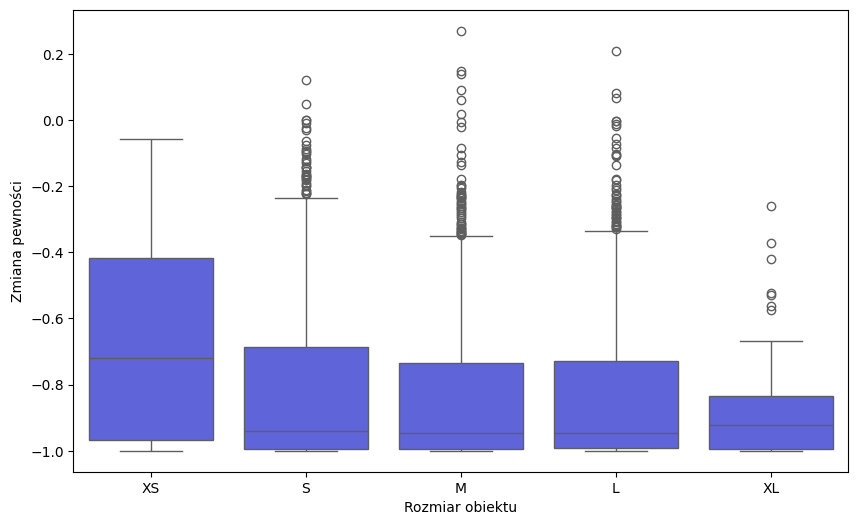
\includegraphics[width=.9\textwidth]{img/size_confidence_exp_shap}
		\caption{SHAP}  \label{rys:size_confidence_mask_shap}
	\end{subfigure}
	\caption{Zmiana pewności przy usunięciu obszarów wyjaśnienia}
	\label{rys:size_confidence_exp}
\end{figure}

\begin{table}[h]
	\centering
	\begin{tabular}{|c|c|c|c|}
		\hline
		\textbf{Rozmiar} & \textbf{GradCAM} & \textbf{LIME} & \textbf{SHAP} \\
		\hline
		\textbf{Mały}    & -0.262645        & -0.658282     & -0.567562     \\
		\hline
		\textbf{Średni}  & -0.242182        & -0.753241     & -0.592994     \\
		\hline
		\textbf{Duży}    & -0.238938        & -0.789269     & -0.590214     \\
		\hline
	\end{tabular}
	\caption{Zmiana pewności przy samym obszarze wyjaśnienia w zależności od rozmiaru obiektu na obrazie}
	\label{tab:size_confidence_exp}
\end{table}

\begin{table}[h]
	\centering
	\begin{tabular}{|c|c|c|c|}
		\hline
		\textbf{Rozmiar} & \textbf{GradCAM} & \textbf{LIME} & \textbf{SHAP} \\
		\hline
		\textbf{Mały}    & 22.7171\%        & 4.0831\%      & 6.6815\%      \\
		\hline
		\textbf{Średni}  & 26.3048\%        & 1.6701\%      & 5.5672\%      \\
		\hline
		\textbf{Duży}    & 25.3555\%        & 0.8689\%      & 4.5814\%      \\
		\hline
	\end{tabular}
	\caption{Procent przypadków, w których pewność się zwiększyła sam obszar wyjaśnienia dla rozmirów}
	\label{tab:size_confidence_exp_percent}
\end{table}

Wyniki analizy zmiany pewności po pozostawieniu jedynie obszarów wyjaśnienia dla różnych wielkości obiektów obrazów przedstawiono na wykresach (Rys. \ref{rys:size_confidence_exp}) oraz w Tabelach \ref{tab:size_confidence_exp} oraz \ref{tab:size_confidence_exp_percent}.

W przypadku GradCAM zmiana pewności modelu po pozostawieniu obszarów wyjaśnień jest najmniejsza dla dużych obiektów.
Spadek pewności jest mniejszy dla większych obiektów, co może sugerować, że GradCAM skuteczniej identyfikuje kluczowe obszary dla większych obiektów, które mają większy wpływ na pewność modelu.
GradCAM osiągnął najwyższy procent przypadków, w których pewność się zwiększyła dla średnich obiektów.
GradCAM wykazuje największą skuteczność dla średnich obiektów w kontekście zwiększania pewności modelu, chociaż różnice pomiędzy kategoriami rozmiarów nie są znaczne.

LIME wykazał największy spadek pewności dla dużych obiektów.
Spadek pewności jest większy dla większych obiektów, co może sugerować, że LIME ma trudności z identyfikacją kluczowych obszarów dla większych obiektów, co skutkuje większym spadkiem pewności modelu.
LIME osiągnął największy procent przypadków, w których pewność się zwiększyła dla małych obiektów.
LIME wykazuje największą skuteczność dla małych obiektów w kontekście zwiększania pewności modelu, co potwierdza jego lepszą zdolność do pracy z mniejszymi obiektami.

SHAP wykazał najmniejszy spadek pewności dla dużych obiektów.
Spadek pewności jest stosunkowo podobny dla wszystkich rozmiarów obiektów, z niewielką tendencją do mniejszego spadku dla większych obiektów, co może sugerować, że SHAP jest bardziej stabilny w identyfikacji kluczowych obszarów niezależnie od wielkości obiektu.

\textbf{Zmiana pewności po usunięciu obszarów wyjaśnień}
\begin{figure}[h]
	\centering
	\begin{subfigure}[b]{0.3\textwidth}
		\centering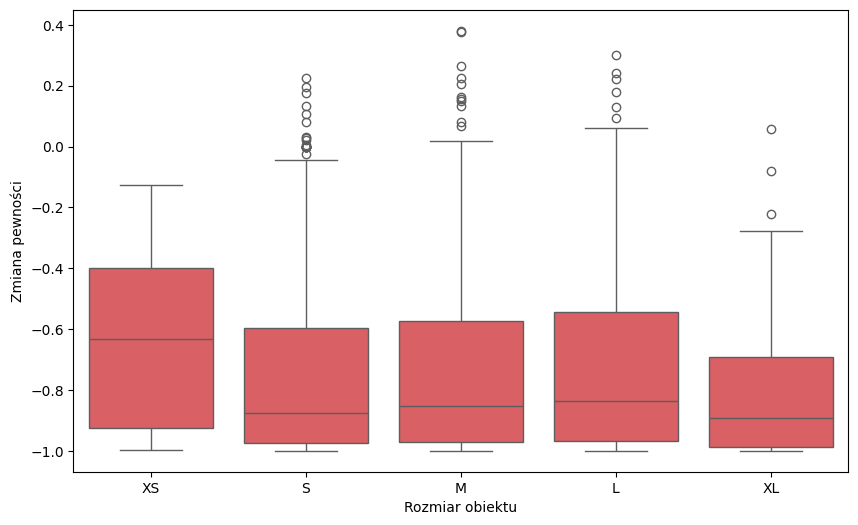
\includegraphics[width=.9\textwidth]{img/size_confidence_no_exp_gradcam}
		\caption{GradCAM}  \label{rys:size_confidence_no_exp_gradcam}
	\end{subfigure}
	\begin{subfigure}[b]{0.3\textwidth}
		\centering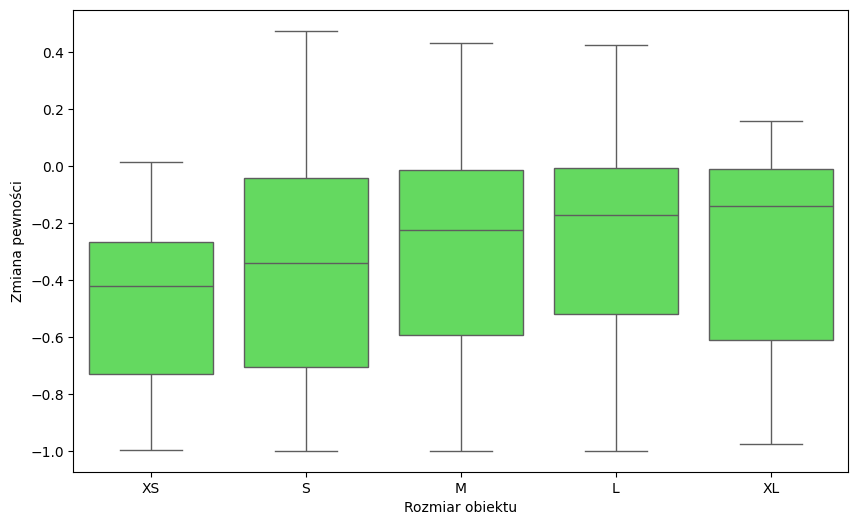
\includegraphics[width=.9\textwidth]{img/size_confidence_no_exp_lime}
		\caption{LIME}  \label{rys:size_confidence_no_exp_lime}
	\end{subfigure}
	\begin{subfigure}[b]{0.3\textwidth}
		\centering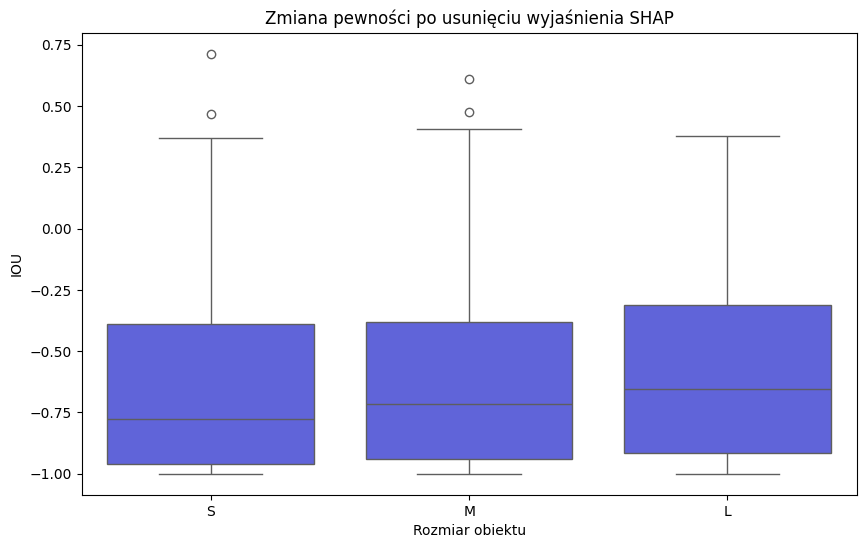
\includegraphics[width=.9\textwidth]{img/size_confidence_no_exp_shap}
		\caption{SHAP}  \label{rys:size_confidence_no_exp_shap}
	\end{subfigure}
	\caption{Zmiana pewności po usunięciu obszatu wyjaśnienia - rozmiar obiektu}
\end{figure}

\begin{table}[h]
	\centering
	\begin{tabular}{|c|c|c|c|}
		\hline
		\textbf{Rozmiar} & \textbf{GradCAM} & \textbf{LIME} & \textbf{SHAP} \\
		\hline
		\textbf{Mały}    & -0.758815        & -0.538989     & -0.658195     \\
		\hline
		\textbf{Średni}  & -0.749968        & -0.382061     & -0.627136     \\
		\hline
		\textbf{Duży}    & -0.732993        & -0.288121     & -0.592250     \\
		\hline
	\end{tabular}
	\caption{Średni spadek po usunięciu obszaru wyjaśnienia dla rozmiarów}
	\label{tab:size_confidence_no_exp}
\end{table}

GradCAM wykazał najmniejszy spadek pewności dla dużych obiektów.
GradCAM lepiej identyfikuje kluczowe obszary na obrazach zawierających większe obiekty, co skutkuje mniejszym spadkiem pewności modelu po ich usunięciu.

LIME wykazał największy spadek pewności dla małych obiektów.
LIME ma trudności z identyfikacją kluczowych obszarów na obrazach zawierających mniejsze obiekty, co prowadzi do większego spadku pewności modelu po ich usunięciu.

SHAP wykazał najmniejszy spadek pewności dla dużych obiektów.
SHAP jest stabilny w identyfikacji kluczowych obszarów niezależnie od wielkości obiektu, co skutkuje mniejszym spadkiem pewności modelu po ich usunięciu.

\vspace{1cm}
Analiza wyników w zależności od wielkości obiektów na obrazach wskazuje na istotne różnice w skuteczności metod XAI.
GradCAM wykazuje najlepsze wyniki dla dużych obiektów, sugerując jego skuteczność w identyfikacji kluczowych obszarów na obrazach zawierających większe obiekty.
LIME natomiast osiąga najniższe wyniki dla dużych obiektów, co może wskazywać na trudności w identyfikacji obszarów istotnych dla klasyfikacji modelu w przypadku większych obiektów.
SHAP wykazuje dobre wyniki dla dużych obiektów, a jego skuteczność jest stosunkowo stabilna dla różnych rozmiarów obiektów.
Te różnice podkreślają znaczenie uwzględniania wielkości obiektu w interpretacji modeli oraz wyboru odpowiedniej metody XAI w zależności od specyfiki danych i celu analizy.
